\chapter{本テンプレートの使い方}
\label{chap:howto}

本章では、本テンプレートの具体的な使用方法を解説する。基本的には、{\tt main.tex} を上から順に修正していけばよいだけ。 


\section{テンプレートの構成}

このテンプレートは、表\ref{tb:files}のファイルで構成されている。

\begin{table}[htbp]
  \caption{構成ファイル}
  \label{tb:files}
  \begin{center}\begin{tabular}{c|l}
    \hline
    ファイル名&用途\\\hline\hline
    {\tt main.tex}&メインのファイル。これを編集していく\\\hline
    {\tt thesis.sty}&論文のスタイルを定義したファイル。基本的には手は加えない\\\hline
    {\tt *.tex}&{\tt main.tex}に{\tt include}されるファイル群\\\hline
    {\tt *.eps}&画像ファイル\\\hline
    {\tt main.bib}&参考文献用のBibTeXファイル\\\hline
    {\tt Makefile}&Makefile。次節以降で説明\\\hline
    {\tt .gitignore}&Git用設定ファイル\\\hline
  \end{tabular}\end{center}
\end{table}

\section{コンパイル}
このテンプレートの\LaTeX ファイルをコンパイルしてPDFファイルを生成するには、ターミナルを開いて以下のようにする。

\begin{itembox}[l]{コマンド実行例}
\begin{verbatim}
% make
\end{verbatim}
\end{itembox}

こうすることで、\verb|platex|コマンド、\verb|pbibtex|コマンド、\verb|platex|コマンド2回、\verb|dvipdfmx|コマンドが全て実行され、{\tt main.pdf}が生成される。

コンパイルによって生成されたファイルを全て消すには、以下のようにする。

\begin{itembox}[l]{コマンド実行例}
\begin{verbatim}
% make clean
\end{verbatim}
\end{itembox}

\section{設定}

以下、{\tt main.tex}に対して行うべき設定を、このファイルの中に書いてある順に沿って説明する。

\subsection{論文全体の言語の設定}
\label{sec:lang}

\begin{itembox}[l]{{\tt main.tex}}
\begin{verbatim}
\japanesetrue	% 論文全体を日本語で書く(英語で書くならコメントアウト)
\end{verbatim}
\end{itembox}

ここでは論文全体の言語を設定する。日本語に設定すれば、『章』『目次』『謝辞』などが日本語で出力されて、行頭のインデントなども日本語の仕様になる。英語にした場合は、これらはそれぞれ『Chapter』『Table of Contents』『Acknowledgment』な体裁になる。インデントも行間も、英語用の設定が適用される。

\verb|\japanesetrue| をコメントアウトしなければ日本語に、コメントアウトすれば英語に設定される。


\subsection{余白の設定}

\begin{itembox}[l]{{\tt main.tex}}
\begin{verbatim}
\bindermode	% バインダ用余白設定
\end{verbatim}
\end{itembox}

このテンプレートの出力はA4用紙。ここではこれの四辺の余白を設定する。

最終的にバインダーで綴じて提出する場合、余白を左右対称にしてしまうと、見かけ上のバランスがとても悪くなる。これを解消するため、あらかじめ左側の余白を大きく取っておく。

\verb|\bindermode| をコメントアウトしなければ左綴じ用の余白に、コメントアウトすれば左右対称の余白に設定される。

両面印刷の場合、偶数ページと奇数ページで余白を広くとるべき側が違うので、\verb|documentclass| でこれを設定する。

\begin{itembox}[l]{{\tt main.tex}}
\begin{verbatim}
% 両面印刷の場合。余白を綴じ側に作って右起こし。
\documentclass[a4j,twoside,openright,11pt]{jreport}
% 片面印刷の場合。
%\documentclass[a4j,11pt]{jreport}
\end{verbatim}
\end{itembox}

両面印刷の場合は \verb|twoside| を使用する。\verb|openright| を使うと章のはじまりが必ず右側のページに来るようになる。

\subsection{論文情報の設定}
\label{sec:meta}

\begin{itembox}[l]{{\tt main.tex}}
\begin{verbatim}
% 日本語情報(必要なら)
\jclass  {修士論文}                             % 論文種別
\jtitle    {修士論文用 \LaTeX\ テンプレート}    % タイトル。改行する場合は\\を入れる
\juniv    {慶應義塾大学大学院}                  % 大学名
\jfaculty  {政策・メディア研究科}               % 学部、学科
\jauthor  {ほげ山 ふう助}                       % 著者
\jhyear  {24}                                   % 令和○年度
\jsyear  {2012}                                 % 西暦○年度
\jkeyword  {\LaTeX、テンプレート、修士論文}     % 論文のキーワード
\jproject{インタラクションデザインプロジェクト} %プロジェクト名
\jdate{2013年1月}

% 英語情報(必要なら)
\eclass  {Master's Thesis}                            % 論文種別
\etitle    {A \LaTeX Template for Master Thesis}      % タイトル。改行する場合は\\を入れる
\euniv  {Keio University}                             % 大学名
\efaculty  {Graduate School of Media and Governance}  % 学部、学科
\eauthor  {Fusuke Hogeyama}                           % 著者
\eyear  {2012}                                        % 西暦○年度
\ekeyword  {\LaTeX, Templete, Master Thesis}          % 論文のキーワード
\eproject{Interaction Design Project}                 %プロジェクト名
\edate{January 2013}
\end{verbatim}
\end{itembox}

ここでは論文のタイトルや著者の氏名などのメタデータを記述する。ここで書いたデータは、表紙とアブストラクトのページに使われる。必ずしも日本語と英語の両方を設定しなければいけないわけではなくて、自分が必要とする方だけ記述すればよい。

タイトルが長過ぎる場合は、表紙やアブストラクトのページでは自動で折り返して出力される。もし改行位置を自分で指定したい場合は、その場所に \verb|\\| を入力する。


\section{出力}

\verb|\begin{document}| から \verb|\end{document}| に記述した部分が、実際に{\tt DVI}(最終的には{\tt PDF})ファイルとして出力される。

\subsection{外部ファイルの読み込み({\tt include})}

出力部分の具体的な説明の前に、外部ファイルを読み込む方法を説明する。

\verb|\begin{document}| から \verb|\end{document}| の間では、\verb|\include| コマンドを使うことで、別の {\tt *.tex} ファイルを読み込ませられる。 

\begin{itembox}[l]{{\tt include}しない場合}
\begin{itembox}[l]{{\tt main.tex}}
\begin{verbatim}
\begin{document}
  \begin{jabstract}
  ほげほげ
  \end{jabstract}
\end{document}
\end{verbatim}
\end{itembox}
\end{itembox}

\begin{itembox}[l]{{\tt include}する場合}
\begin{minipage}{0.5\hsize}
\begin{itembox}[l]{{\tt main.tex}}
\begin{verbatim}
\begin{document}
\chapter{序論}
\label{chap:introduction}

論文は序論のようなもので始める。タイトルは序論でも序言でもはじめにでもいいけど、『序論』で始めたら『結論』で終わり、『序言』で始めたら『結言』で終わるようにする。『はじめに』なら『おわりに』で終わる。『序論』で始まって『おわりに』でおわるとか、そういうちぐはぐなのはだめ。

ここでは序論として書く。序論では、研究の背景やら目的やらを書くのが普通。今はテンプレートの説明なので、大して書くことは無い。

\newpage

\section{本研究に至る背景}

私たちはモノを使用することで充実した生活を享受している。そのため、自身のニーズに合致するモノを多く持っている程、生活が充実する。しかし、それらが物体であるが故に、生活の邪魔となったり、使用後に片付けなくてはならなかったりと、不快感や煩わしさを引き起こす原因となる事も多々ある。そのため、部屋に配置するモノを必要最小限に抑え、生活を簡素化することは、最近支持を得られるようになってきた。

生活を簡素化するためにモノを排除する際、機能充実を取るか、不快感や煩わしさの解消を取るかのトレードオフとなる。しかし、モノによっては、この二択を選択することが困難な場合も存在する。

そこで、拡張現実技術(AR)を用いることで、簡素化をしながらも、生活に要するモノを仮想的に再現することを考えた。物理的に依存関係を持たないモノであれば、ARを用いて環境を再現することが可能となる。よって、本研究では、部屋内のモノをARで再現し、仮想的に代替することにより、生活の簡素化と機能充実の両方を実現するシステムについて提案し、考察する。

\section{提案目的}

日常的に利用している部屋の要素を部屋内のモノをARで再現し、仮想的に代替することにより、生活の簡素化と機能充実を両立し、利便化を図ることが本研究の目的である。

\section{本論文の構成}

\ref{chap:suggestion}章では、簡素化支援システムの提案と具体例についての考察を行う。3章では、実際に制作した簡素化支援システムについての詳細について説明する。4章では、2章・3章を元に、簡素化支援システムを運用しての考察と問題点について述べる。5章では、関連システムを例示し、簡素化支援システムとの相違点や参考点をまとめる。6章では、これまでの考察を元に、簡素化支援システムの今後の展望について述べる。最後に、7章では、全体を通しての総括を行う。
 % 01.texをinclude
\end{document}
\end{verbatim}
\end{itembox}
\end{minipage}
\begin{minipage}{0.5\hsize}
\begin{itembox}[l]{{\tt 01.tex}}
\begin{verbatim}
\begin{jabstract}
ほげほげ
\end{jabstract}
\end{verbatim}
\end{itembox}
\end{minipage}
\end{itembox}

{\tt include}しない場合とする場合を比較するとこのとおり。どちらも出力結果は一緒。{\tt include}する場合は、読み込ませたい箇所に、読み込ませたい{\tt *.tex}ファイルの名前を、拡張子を除いて \verb|\include| コマンドで書けばよい。

\verb|\include| コマンドを用いるか用いないかは、たぶん文書量や個人の好みに依る。例えば章ごとに別のファイルにしておけば、修正箇所を探すときの手間が多少は省けるかもしれない。Gitで人と共有しつつ校正を頼むときにもファイルが分かれていたほうがコンフリクトを起こしにくい。


\subsection{表紙の出力}

\begin{itembox}[l]{{\tt main.tex}}
\begin{verbatim}
\ifjapanese
  \jmaketitle    % 表紙(日本語)
\else
  \emaketitle    % 表紙(英語)
\fi
\end{verbatim}
\end{itembox}

最初に、表紙を出力する。

\verb|\jmaketitle| が実行されると日本語の表紙が、\verb|\emaketitle| が実行されると英語の表紙がそれぞれ出力される。日本語の表紙には、第\ref{sec:meta}節で設定したうちの日本語の情報が、英語の表紙には同節で設定したうち英語の情報が、それぞれ参照されて、表記される。

デフォルトでは第\ref{sec:lang}説で設定した言語の表紙のみが出力されるようになっている。

\subsection{アブストラクトの出力}

\begin{itembox}[l]{{\tt main.tex}}
\begin{verbatim}
% ■ アブストラクトの出力 ■
%	◆書式:
%		begin{jabstract}〜end{jabstract}	:日本語のアブストラクト
%		begin{eabstract}〜end{eabstract}	:英語のアブストラクト
%		※ 不要ならばコマンドごと消せば出力されない。



% 日本語のアブストラクト
\begin{jabstract}

テンプレートの説明を、テンプレート自身を使って説明する。これは @kurokobo による卒業論文のための\LaTeX テンプレートを修士論文用に改造し、さらにUTF-8化やMakefile等の添付をしたものである。

この部分には一般には論文のアブストラクトを書く。日本語のアブストラクトを書きたいなら、\verb|\begin{jabstract}| と \verb|\end{jabstract}| の間に文章を書けば、今のこのページのように体裁が勝手に整って出力される。英語のアブストラクトは \verb|\begin{eabstract}| と \verb|\end{eabstract}| の間に書けば、次ページのような体裁で出力される。

両方を書けば、日本語と英語の両方のアブストラクトが並んで出力される(この文書はサンブルなので両方書いてある)。ページ順序は、コマンドを書いた順序の通り。どちらか一方のみを出力したい場合は、不要な方をコマンド自体を含め削除する。

このあたりの詳細もあとで書く。基本的には、{\tt main.tex}を上から順にいじっていけばできるはず。

\end{jabstract}

	% アブストラクト。要独自コマンド、include先参照のこと
\end{verbatim}
\end{itembox}

表紙の次は、アブストラクト。

アブストラクトを出力するには、出力したい位置に、指定のコマンドを用いて文章を書き下せばよい。{\tt main.tex}に直接書いてもよいし、先述した \verb|\include| コマンドを利用して{\tt include}してもよい。

\verb|\begin{jabstract}| から \verb|\end{jabstract}| の間に書いた文章が日本語のアブストラクトとして、\verb|\begin{eabstract}| から \verb|\end{eabstract}| の間に書いた文章が英語のアブストラクトとして、それぞれ独立したページに出力される。

アブストラクトのページには、論文のタイトルやキーワードなどが、第\ref{sec:meta}節で設定した情報をもとにして自動で表記される。

日本語か英語のどちらか一方のみでよい場合は、不要な言語の方のコマンドを削除すればよい。これは、\verb|\begin| と \verb|\end| というコマンド自身も含めて削除する、ということで、\verb|\begin| と \verb|\end| の間を空っぽにするという意味ではないので注意。



\subsection{目次類の出力}
\label{sec:toc}

\begin{itembox}[l]{{\tt main.tex}}
\begin{verbatim}
\tableofcontents	% 目次
\listoffigures		% 表目次
\listoftables		% 図目次
\end{verbatim}
\end{itembox}

アブストラクトの次に、目次。文書の目次、図の目次、表の目次の三種類。

目次類を出力するには、出力したい位置に指定のコマンドを書けばよい。

これらのコマンドは、コンパイル時点での一時ファイル\footnote{{\tt *.toc}、{\tt *.lof}、{\tt *.lot}}の情報を、目次として体裁を整えて出力するもの。一時ファイルは、\verb|\begin{document}| から \verb|\end{document}| の間の章や節、図や表をコンパイルするときに、ついでに情報を取得しておいて生成される。

つまり気をつけなければいけないのは、コンパイルを一回しただけでは、一時ファイルが最新の状態に更新されるだけで、肝心の目次は正しい情報では出力されないということ。目次類を正しい情報で出力するには、最低二回のコンパイルが必要。一回目のコンパイルで一時ファイルが最新の情報に更新されて、二回目のコンパイルで初めて、その最新の一時ファイルの情報をもとに目次が出力される。

だから、文書に何らかの修正をして保存したあとは、最低でも二回、連続してコンパイルしないといけないことに注意する。

図や表を一つも使用していない場合は、目次名のみが書かれた空白のページが出力される。もしこれが不要な場合は、該当するコマンドをコメントアウトすればよい。


\subsection{本文の出力}

\begin{itembox}[l]{{\tt main.tex}}
\begin{verbatim}
\chapter{序論}
\label{chap:introduction}

論文は序論のようなもので始める。タイトルは序論でも序言でもはじめにでもいいけど、『序論』で始めたら『結論』で終わり、『序言』で始めたら『結言』で終わるようにする。『はじめに』なら『おわりに』で終わる。『序論』で始まって『おわりに』でおわるとか、そういうちぐはぐなのはだめ。

ここでは序論として書く。序論では、研究の背景やら目的やらを書くのが普通。今はテンプレートの説明なので、大して書くことは無い。

\newpage

\section{本研究に至る背景}

私たちはモノを使用することで充実した生活を享受している。そのため、自身のニーズに合致するモノを多く持っている程、生活が充実する。しかし、それらが物体であるが故に、生活の邪魔となったり、使用後に片付けなくてはならなかったりと、不快感や煩わしさを引き起こす原因となる事も多々ある。そのため、部屋に配置するモノを必要最小限に抑え、生活を簡素化することは、最近支持を得られるようになってきた。

生活を簡素化するためにモノを排除する際、機能充実を取るか、不快感や煩わしさの解消を取るかのトレードオフとなる。しかし、モノによっては、この二択を選択することが困難な場合も存在する。

そこで、拡張現実技術(AR)を用いることで、簡素化をしながらも、生活に要するモノを仮想的に再現することを考えた。物理的に依存関係を持たないモノであれば、ARを用いて環境を再現することが可能となる。よって、本研究では、部屋内のモノをARで再現し、仮想的に代替することにより、生活の簡素化と機能充実の両方を実現するシステムについて提案し、考察する。

\section{提案目的}

日常的に利用している部屋の要素を部屋内のモノをARで再現し、仮想的に代替することにより、生活の簡素化と機能充実を両立し、利便化を図ることが本研究の目的である。

\section{本論文の構成}

\ref{chap:suggestion}章では、簡素化支援システムの提案と具体例についての考察を行う。3章では、実際に制作した簡素化支援システムについての詳細について説明する。4章では、2章・3章を元に、簡素化支援システムを運用しての考察と問題点について述べる。5章では、関連システムを例示し、簡素化支援システムとの相違点や参考点をまとめる。6章では、これまでの考察を元に、簡素化支援システムの今後の展望について述べる。最後に、7章では、全体を通しての総括を行う。
	% 本文1

\chapter{提案}
\label{chap:suggestion}

この章では、ARを用いた生活の簡素化支援システムについて提案し、その具体的な用途について、各例ごとに考察する。

\newpage

\section{ARを用いたモノの仮想的代替による簡素化支援システムの提案}
\label{chap:suggestionDetail}

\subsection{概要}

簡素化支援システムとは、生活の簡素化のために排除したモノをARで仮想的に再現し、その代替として利用することで、簡素化前と同程度、或いはそれ以上に充実した機能を得ることができる、実世界の一部を代替するインターフェースである。

なお、ARでの仮想的な代替を実現するため、常にARデバイスを使用し続ける事を前提としている。

\subsection{仮想的な代替が可能なモノ}

仮想的な代替には、それが可能なモノと不可能なモノが存在する。人や物体の支えとなるモノや、温度を制御する機能を持つモノなど、対象のモノがその場になくては役割を果たせないものか否かで判別する。下記の表は、一般的な部屋内のモノについて、その場になくても役割を果すものとそうでないものを分類したものである。

\begin{table}[htbp]
    \caption{対象のモノがその場に必要なものか否か}
    \label{tb:mono}
    \begin{center}\begin{tabular}{c|c}
      \hline
      必要なもの&机・椅子・本棚・タンス・冷蔵庫・洗濯機・エアコン etc.\\\hline
      必要でないもの&テレビ・時計・PCディスプレイ・カレンダー・ポスター etc.\\\hline
    \end{tabular}\end{center}
\end{table}

簡素化支援システムでは、後者に分類された物体を実世界で配置する代わりに、ARを用いて仮想的に表示することにより、生活の機能充実を損なわずに、実世界の空間の簡素化を実現する。

\subsection{使用するARデバイスについて}
\label{chap:ARdevice}

簡素化支援システムは、日常的に利用される前提のため、デバイスについても同様に日常的に使用できることが条件となる。現段階では、ARグラスがその条件を満たす技術であると推察する。ARグラスとは、実世界に重ねて描画できるグラフィックデバイスで、実世界を認識して得た情報を元に、実世界に重ねて表示をする眼鏡型のデバイスである。代表的なARグラスとして、Hololens\footnote{Microsoft Hololens: \url{https://www.microsoft.com/ja-jp/hololens}(accessed 2021-01-26)}、Magic leap 1\footnote{Magic leap 1: \url{https://www.magicleap.com/ja-jp/magic-leap-1} (accessed 2021-01-26)}、Nreal light\footnote{Nreal light: \url{https://www.nreal.ai/light/} (accessed 2021-01-26)}などがある。いずれもPCを必要とせず、スタンドアロンで動作する。空間に対する位置・角度などを検知できるため、6DoF(six degrees of freedom)に対応しており、高い没入感を得ることができる。

\newpage

\section{簡素化支援システムの具体的なシナリオの考察}

ここでは、\ref{chap:suggestionDetail}にて挙げた生活の簡素化支援システムについて、より具体的なシナリオを交えた上で、多角的に考察する。

\subsection{部屋の空間の確保と機能性の拡張}

\ref{tb:mono}で提示したモノを部屋から排除することにより、実世界に空間を確保をすることができる。確保した空間には、ARで再現したモノを表示するが、状況に応じて非表示にしたり、別のモノを表示することも可能なため、より自由度の高い空間として利用することが可能である。また、ARによって仮想的に表示しているため、物理法則に囚われない表示をすることも可能である。壁や天井などは使用されていないスペースとなっている場合が多いが、そういったスペースも有効活用できる。

また、実際には配置することが難しいモノを配置することで、部屋内の機能をより充実させることができる。例えば、スマホウィジットに代表される、時間、天気やカレンダー、todo、体調状態、メモなどを配置することで、スマートフォンのホーム画面のように使用できる(図\ref{fig:widget})。なお、スマートフォンでの時刻や日付の確認が容易になった現代でも、カレンダーや時計を部屋に配置する事と同様に、これらの情報を実世界上で見られるようにすることで、モノの位置を、部屋内の絶対位置やモノ同士の相対的な位置関係といった二次的な情報に紐づけて記憶することができ、欲しい情報を瞬時に獲得、もしくは機能を利用する事ができるのではないかと推察する。

\begin{figure}[htbp]
    \begin{center}
       \fbox{\includegraphics[width=60mm]{images/living_room_01.png}}
    \end{center}
    \caption{通常の部屋環境のイメージ}
    \label{fig:normal-room}
  \end{figure}

\begin{figure}[htbp]
    \begin{minipage}{0.5\hsize}
      \begin{center}
        \fbox{\includegraphics[width=60mm]{images/living_room_02.png}}
      \end{center}
      \label{fig:bigTV}
      \caption{テレビを仮想的に代替したイメージ}
    \end{minipage}
    \begin{minipage}{0.5\hsize}
      \begin{center}
        \fbox{\includegraphics[width=60mm]{images/living_room_03.png}}
      \end{center}
      \caption{部屋をスマホのホーム画面のように使用できるイメージ}
      \label{fig:widget}
    \end{minipage}
\end{figure}

\subsection{同様の環境を他所で再現}

自身が身を置く場所は常に一定ではなく、自宅の部屋以外にもオフィスやカフェ、ホテルなどの場所に身を置くこともある。その際に、本システムを利用する事で、普段とは違う場所でも自室の環境を再現することができる。

また、他所の部屋環境を自身の部屋環境として再現することも可能である。オフィスや映画館など、シチュエーションに応じたモノの再現が可能なため、より個人の充実に適した環境を用意することができる。

\subsection{物体の管理や更新、カスタマイズ}

仮想的なモノは実体を持たないので、購入や修理などのコストがかからない。また、物体の更新にも物理的なコストは掛からないので、色や形、大きさまで、自由にカスタマイズすることができる。

	% 本文2

\chapter{実装}
\label{chap:implementation}

本章では、前章で提案した生活の簡素化支援システムの実装に関する要件と設計について述べる。

\newpage

\section{機能}
本システムでは、部屋内のモノをARで再現し、仮想的に代替することで、本来利用している部屋と同程度の環境の再現を行う。どのような部屋に対しても同様の環境を作ることができる事を条件とし、マーカーに対してモノを表示する、画像認識型ARを採用した。部屋内に配置されたマーカーを認識することにより、その位置を中心として、対応する3Dないし2Dのモノを表示する。部屋にマーカーを貼るだけで環境の準備ができ、表示位置の再設定や、他所への持ち運びなども容易である。

\section{基本構成}

本システムのデバイスには、Microsoft社の提供するHololensを使用している。スタンドアロンで動作するARグラスであり、着用したままであっても、日常を過ごす事ができる。Hololens上で動作するソフトウェアの実装には、Unity\cite{unity}, vuforia\cite{vuforia}を使用した。予めマーカー画像を準備した部屋内でHololensを装着し、本システムを起動することで動作する。

マーカーには、processingで生成したランダムな画像を使用した。

\begin{figure}[htbp]
  \begin{minipage}{0.5\hsize}
    \begin{center}
      \fbox{
\includegraphics[width=60mm]{images/marker.png}}
    \end{center}
    \caption{使用したマーカー}
  \end{minipage}
  \begin{minipage}{0.5\hsize}
    \begin{center}
      \fbox{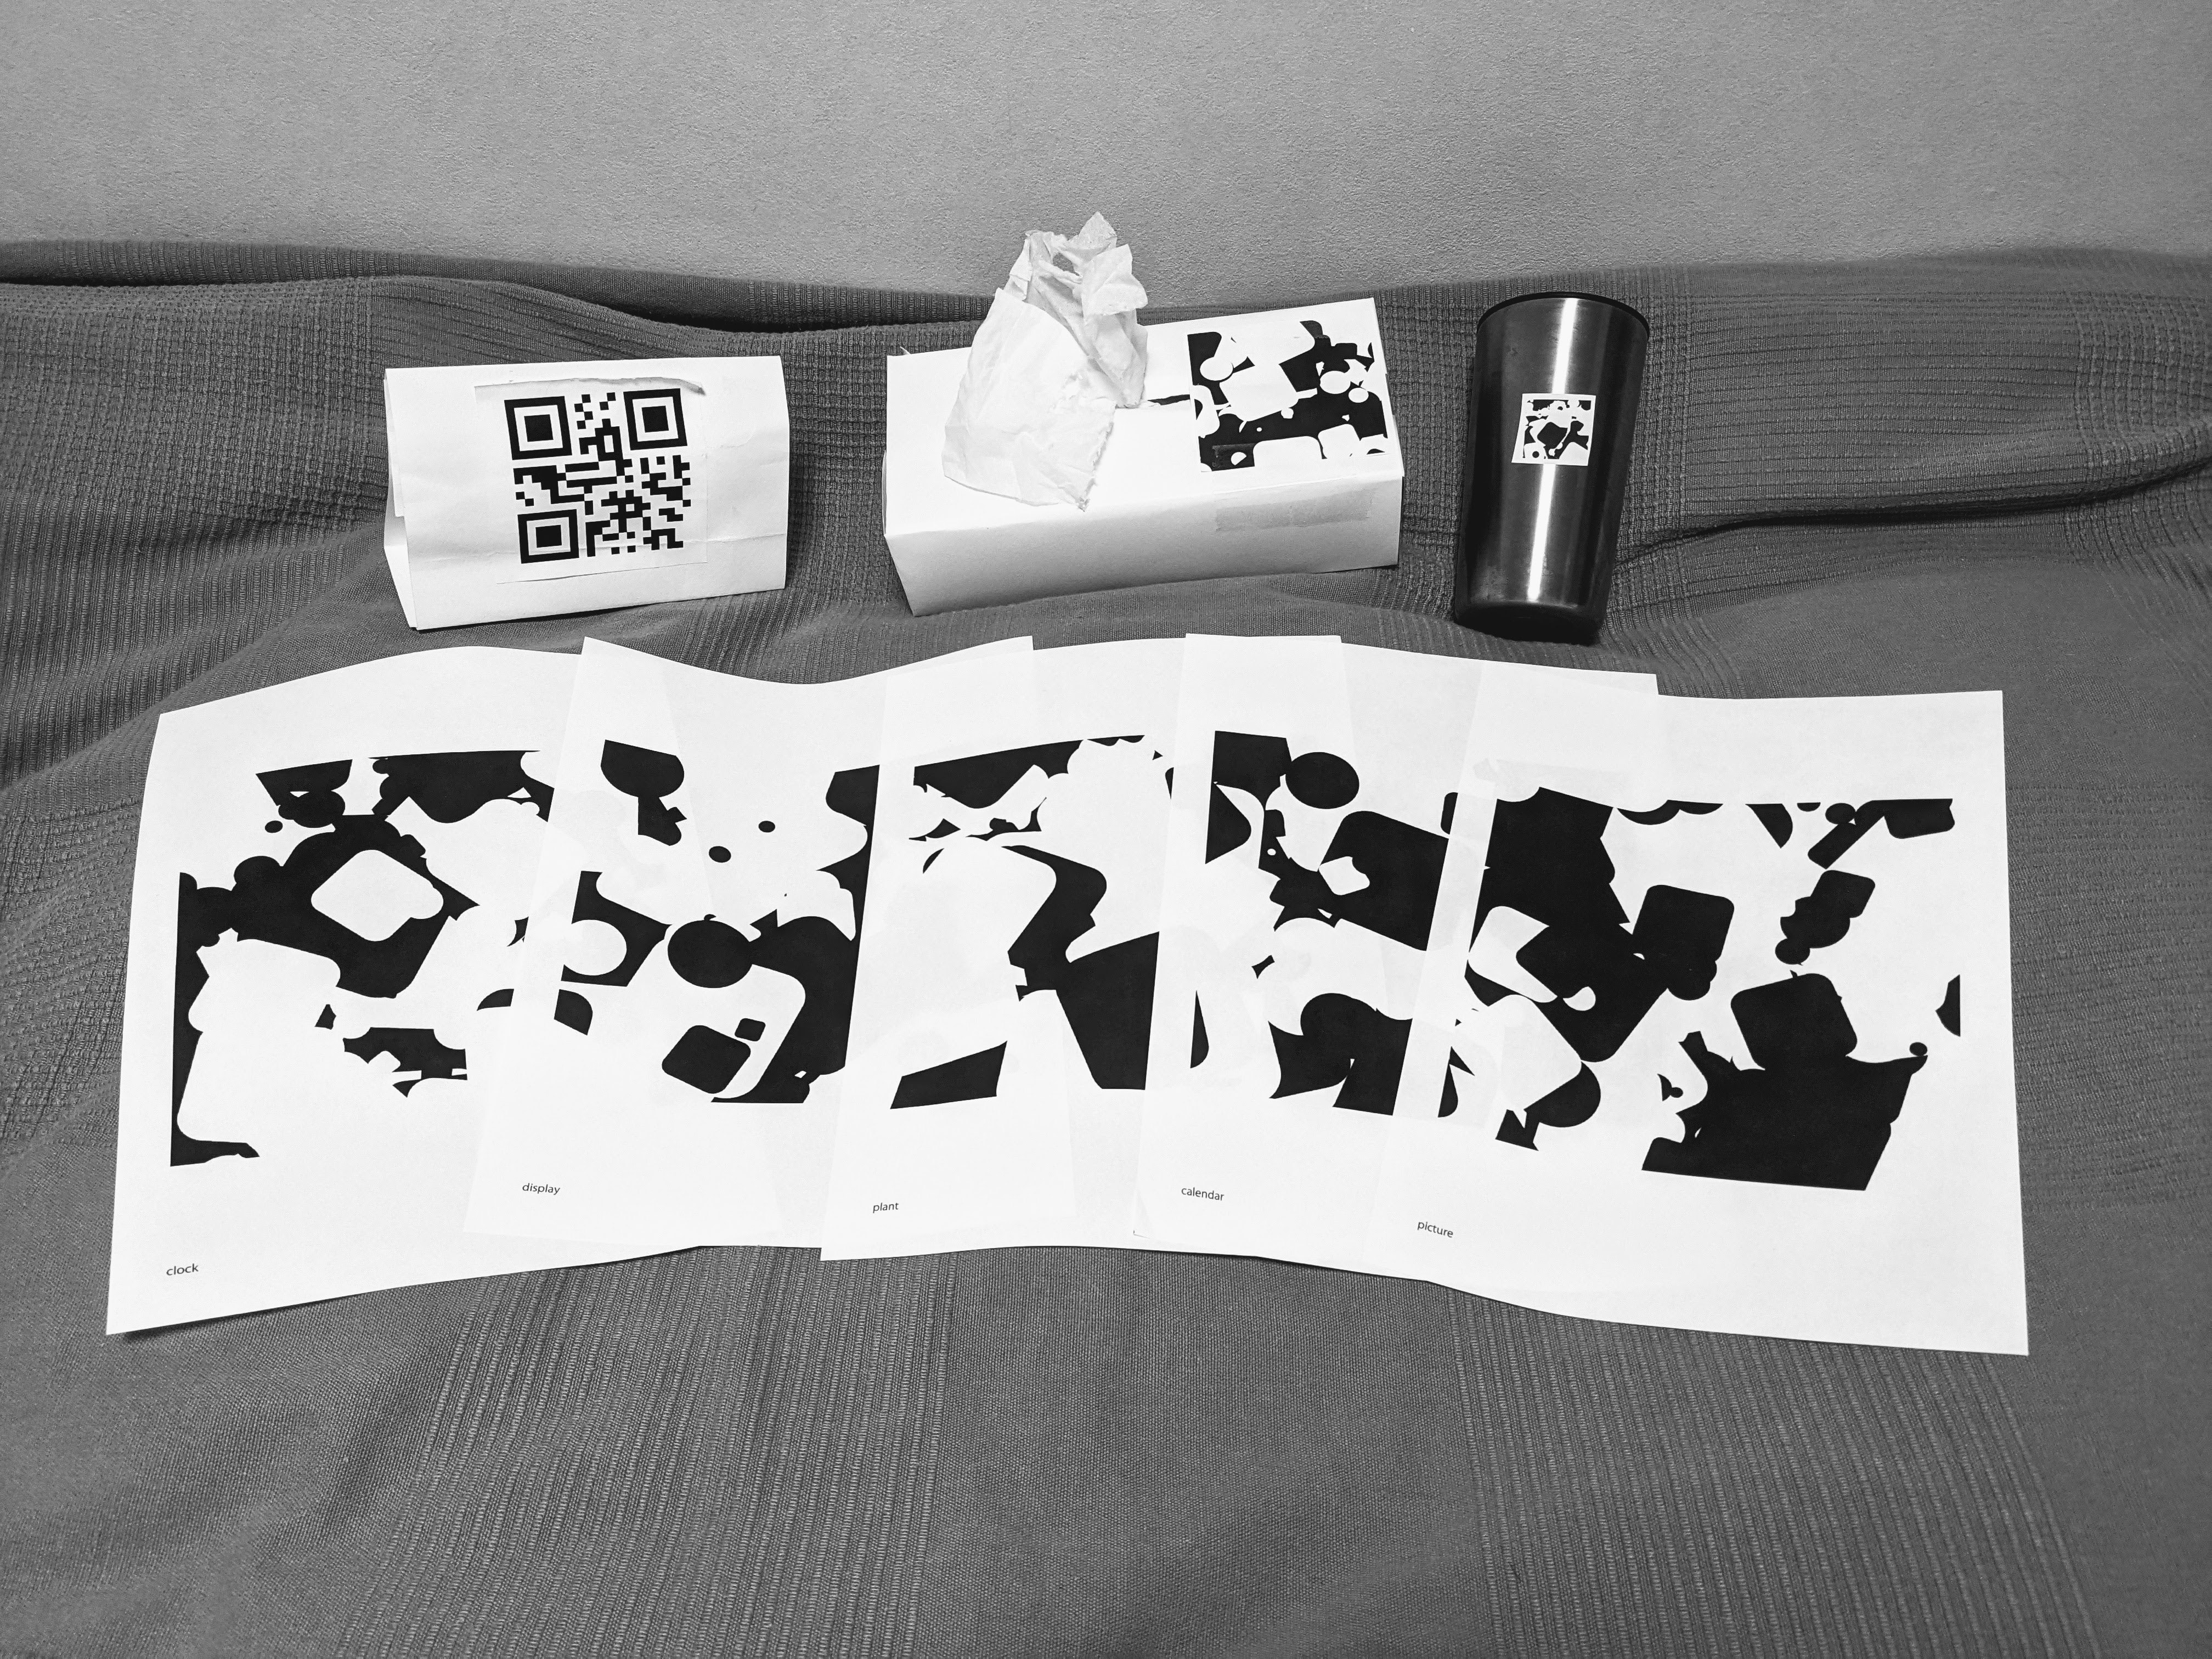
\includegraphics[width=60mm]{images/markers.jpg}}
    \end{center}
    \caption{適用したマーカー}
  \end{minipage}
\end{figure}


\section{実装}

\subsection{準備}

本提案の要件を最大限に反映するため、空き部屋となっているアパートの一室にてシステムを運用した。システム運用時には、物を置くための机一つを持ち込み、その他は、アパートに備え付けられたもののみがある状態とした。

本システムでは、絵画、カレンダー、壁掛け時計、ディスプレイ、植物、ティッシュの外箱、タンブラー、デジタル時計の合計8つのサンプルコンテンツを用意した。

絵画、カレンダー、壁掛け時計、ディスプレイに対応する四つのマーカーは、一般的な配置場所通り、壁に配置した。また、植物に対応したマーカーは、ARで代替されたの観賞用インテリアの新たな試みとして、壁に配置した。

ティッシュの外箱は、白の用紙で覆ってパッケージが見えない状態にし、マーカー画像を貼り付けた。デジタル時計は、時計そのものではなく、折って三角柱状にした物にマーカーを貼り付けた。ARグラスを通して確認することで、デジタル時計が表示され、その機能を果たす形式となっている。タンブラーには、内容物に対応したパッケージが表示されるマーカーを貼った。

\begin{figure}[htbp]
  \begin{center}
     \fbox{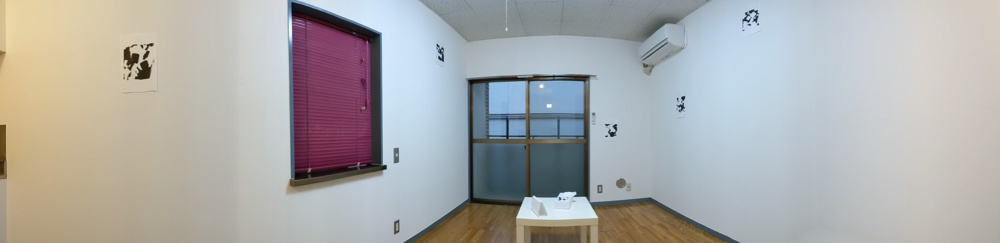
\includegraphics[width=100mm]{images/room_panorama.jpg}}
  \end{center}
  \caption{システムを運用した部屋のパノラマ}
  \label{fig:sample1}
\end{figure}

\subsection{システムの運用}

Hololensを装着し、本システムを起動する事で、hololensに付いているカメラの映像の画像認識が開始される。マーカーを注視する事で、対象のマーカーが認識され、そこに対象のコンテンツが表示される。コンテンツはマーカーに追従するため、マーカーの付いている物体を移動しても問題はない。

\begin{figure}[htbp]
  \begin{minipage}{0.5\hsize}
    \begin{center}
      \fbox{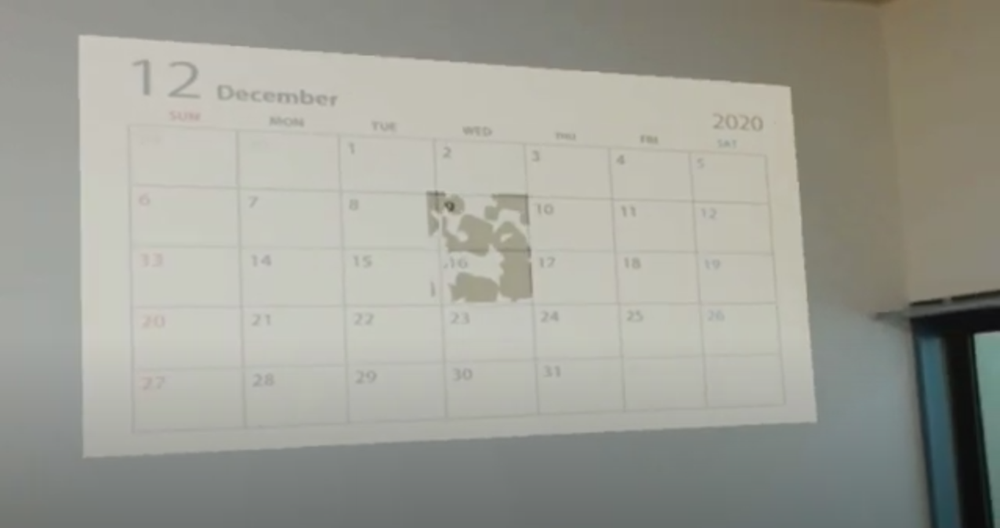
\includegraphics[width=60mm]{images/test_calendar.png}}
    \end{center}
    \caption{仮想的に代替したカレンダー}
  \end{minipage}
  \begin{minipage}{0.5\hsize}
    \begin{center}
      \fbox{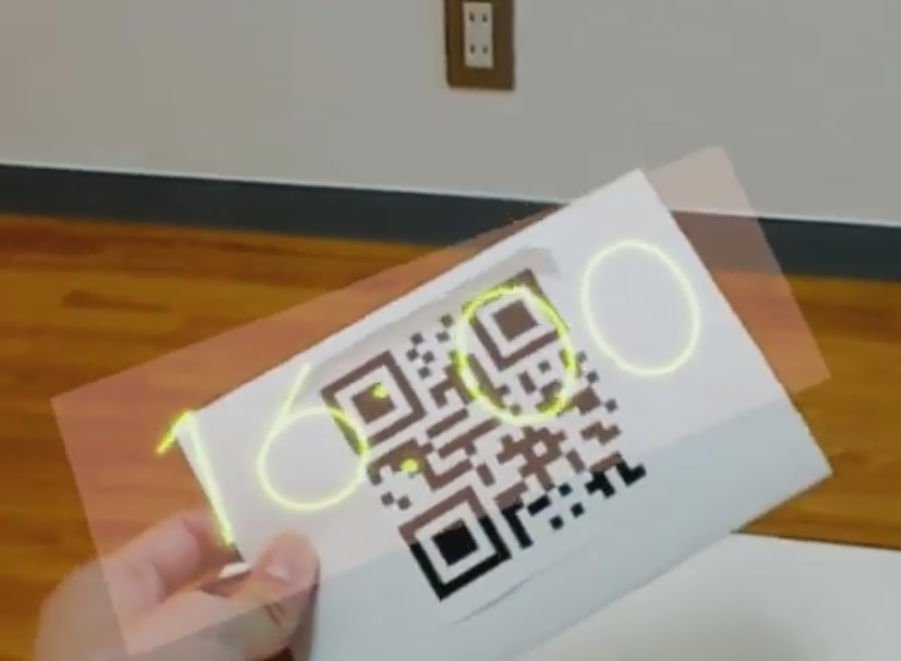
\includegraphics[width=60mm]{images/test_digital_clock.png}}
    \end{center}
    \caption{仮想的に代替したデジタル時計}
  \end{minipage}
\end{figure}

	% 本文3

\chapter{システムの評価と考察}
\label{chap:systemEvaluation}

本章では、前章で実装したシステムを実際に運用した上での考察と問題点について述べる。

\newpage

\section{システムを運用しての考察}

システムの運用時、机以外に何も配置していない環境であったため、窮屈さや煩雑さはなかった。その上で、動画や観葉植物、時計などの機能を得られたため、実世界のモノの少なさに対して、十分な充実感を得ることができた。また、仰向けの状態で動画を鑑賞したいと考えた際も、マーカーを壁から天井に移動するだけで、楽な体勢にて鑑賞することが出来たため、体験の面では、従来よりも満足度は高いと感じた。今後、マーカーを使用しなくとも空間上に意図した形式でモノを配置することが容易になれば、より満足度の高い鑑賞体験ができるのではないかと推察する。

一方で、デバイスの認識精度やスペック上に問題点があり、AR上のモノを正常に使用できない場面が多々あった。本システム上の問題点に関しては後述するが、AR上のモノという、直観ではどうしても解決できない不具合が発生した際、実世界のモノの代替である事もあり、スマートフォンやPC上での不具合よりも強く煩わしさを感じた。AR上での動作が安定するまでの間は、不具合が起こる可能性を加味した運用をすることが重要だと考える。

\section{問題点}

\subsection{マーカーの認識制度}

システムを運用した際、フレームレートの大幅な低下や位置ずれなどが発生した。これらは主にマーカー形状と運用環境の明るさの二点が原因であると類推される。

本システムに利用したマーカーは、自作のアルゴリズムによって生成された画像であった。ランダムな大きさ・位置・角度の円形ないし四角形の領域を、白黒で交互に塗りつぶすことで生成していた。システム制作に使用したvuforiaのマーカー評価では、最大点を記録していたが、単純図形のみで構成した画像であったため、特徴点の数が少なく、結果的に認識精度の低下に繋がったと推察する。また、画像認識によってコンテンツの表示位置を決定しているため、運用環境での明るさが精度に影響する場合がある。運用した日が曇りであったこと、シーリングライトの光量が少なかったことなどから、認識精度を保てなかった可能性がある事が考えられる。

\subsection{デバイスの物理的問題点}

本システムでは、日常的にARグラスを付け続ける事を前提としているが、デバイスの重さと視野角の狭さは、日常的な生活をする上で大きな負担となる。将来的にARグラスを日常利用する上で、軽量化と視野角の拡大は必要な改善である。
	% 本文4
\end{verbatim}
\end{itembox}

目次に続いて、論文のメイン、本文を記述する。アブストラクトと同様で、{\tt main.tex}に直接書くか、\verb|\include| コマンドを利用して別に用意したファイルを{\tt include}する。

本文の書き方は、第\ref{chap:latex}章で詳しく説明する。


\subsection{謝辞の出力}

\begin{itembox}[l]{{\tt main.tex}}
\begin{verbatim}
\begin{acknowledgment}

    本論文を執筆するにあたり、ご指導いただきました増井俊之教授に、心から感謝申し上げます。不器用なために情報共有の段取りが悪くなってしまった中でも、終始的確にご指示やアドバイスをいただいたことで、本研究を進行することができました。
    
    また、アイデアや本論文の構成にご助言くださいました、左治木隆成氏、田中優氏、二塚康平氏をはじめとする、増井研究会の皆様にも、感謝の意を表します。

\end{acknowledgment}
	% 謝辞。要独自コマンド、include先参照のこと
\end{verbatim}
\end{itembox}

本文のあとには、謝辞を出力する。\verb|begin{acknowledgment}| から \verb|end{acknowledgment}| の間に書いた文章が、謝辞として独立したページに出力される。アブストラクトや本文と同じで、{\tt main.tex}に直接書いてもよいし、\verb|\include| コマンドを利用して{\tt include}してもよい。


\subsection{参考文献の出力}

\begin{itembox}[l]{{\tt main.tex}}
\begin{verbatim}
\include{91_bibliography}	% 参考文献。要独自コマンド、include先参照のこと
\end{verbatim}
\end{itembox}

謝辞に続いて、参考文献を出力する。

参考文献リストは、\verb|\begin{bib}| から \verb|\end{bib}| の間に、\verb|\bibitem| コマンドを使って書く。

BibTeXを使う場合は、以下のようにする。

\begin{itembox}[l]{{\tt 91\_bibliography.tex}}
\begin{verbatim}
\begin{bib}[100]
\bibliography{main}
\end{bib}
\end{verbatim}
\end{itembox}

こうすると、\verb|main.bib|から使用した参考文献のみを抽出して出力してくれる。\verb|main.bib|の中身は以下のようになっていて、気の利いた論文検索サイトであればBibTeXをコピペできるようになっているので簡単に作れるはず。


\begin{itembox}[l]{{\tt 91\_bibliography.tex}}
\begin{verbatim}
@article{hoge09,
    author  = "ほげ山太郎 and ほげ山次郎",
    yomi    = "ほげやまたろう",
    title   = "ほげほげ理論のHCI分野への応用",
    journal = "ほげほげ学会論文誌",
    volume  = "31",
    number  = "3",
    pages   = "194-201",
    year    = "2009",
}
@inproceedings{hoge08,
    author     = "Taro Hogeyama and Jiro Hogeyama",
    title      = "The Theory of Hoge",
    booktitle  = "The Proceedings of The Hoge Society",
    year       = "2008"
}
\end{verbatim}
\end{itembox}


以下は、BibTeXを使わないで手で書く例。

\begin{itembox}[l]{{\tt 91\_bibliography.tex}}
\begin{verbatim}
@article{hoge09,
    author  = "ほげ山太郎 and ほげ山次郎",
    yomi    = "ほげやまたろう",
    title   = "ほげほげ理論のHCI分野への応用",
    journal = "ほげほげ学会論文誌",
    volume  = "31",
    number  = "3",
    pages   = "194-201",
    year    = "2009",
}
@inproceedings{hoge08,
    author     = "Taro Hogeyama and Jiro Hogeyama",
    title      = "The Theory of Hoge",
    booktitle  = "The Proceedings of The Hoge Society",
    year       = "2008"
}
\end{verbatim}
\end{itembox}


英語の文献の場合、慣例的に書誌名をイタリック体にすることが多いらしい。

\begin{itembox}[l]{{\tt 91\_bibliography.tex}}
\begin{verbatim}
\begin{bib}[100]
\begin{thebibliography}{#1}
% \bibitem{参照用名称}
%   著者名: 
%   \newblock 文献名,
%   \newblock 書誌情報,出版年.

\bibitem{hoge09}
  ほげ山太郎,ほげ山次郎:
  \newblock ほげほげ理論のHCI分野への応用,
  \newblock ほげほげ学会論文誌,Vol.31,No.3,pp.194-201,2009.

\bibitem{hoge08}
  Taro Hogeyama, Jiro Hogeyama:
  \newblock The Theory of Hoge,
  \newblock {\it The Proceedings of The Hoge Society}, 2008.
\end{thebibliography}
\end{bib}
\end{verbatim}
\end{itembox}

\verb|\bibitem| コマンド中、参照用名称は、本文から参考文献を参照するときに使うので、忘れずに書いておく。参照文献を本文中に参照するときには、\verb|\cite{参照用名称}| のように書けばよい。例えば、この文の末尾には \verb|\cite{hoge09}| と書いてあるので、自動で対応する番号が振られる\cite{hoge09}\cite{hoge08}。

参考文献リストの番号付けと、本文で参照したときの番号の挿入は、全部が自動で行われる。ただしこれも、第\ref{sec:toc}節で説明した目次の出力と同じで、一時ファイルを生成してからの挿入なので、正しく出力するには最低でも二回のコンパイルが必要。BibTeXを使用する場合は、\verb|platex|コマンドのあと\verb|pbibtex|コマンドを実行し、さらに2回\verb|platex|コマンドを実行するといいらしい。



\subsection{付録の出力}

\begin{itembox}[l]{{\tt main.tex}}
\begin{verbatim}
\appendix
\include{92_appendix}		% 付録
\end{verbatim}
\end{itembox}

必要であれば、論文の最後には付録を出力する。

\verb|\appendix| コマンド以降に書いたものは、すべて付録として扱われる。付録部分の書き方は通常の本文とまったく同じで、\verb|\appendix| コマンド以降に書くだけで勝手に付録用の体裁で出力される。
